\documentclass[tikz,border=8pt]{standalone}

\usepackage[T1]{fontenc}
\usepackage{lmodern}
\usetikzlibrary{arrows.meta}

\begin{document}
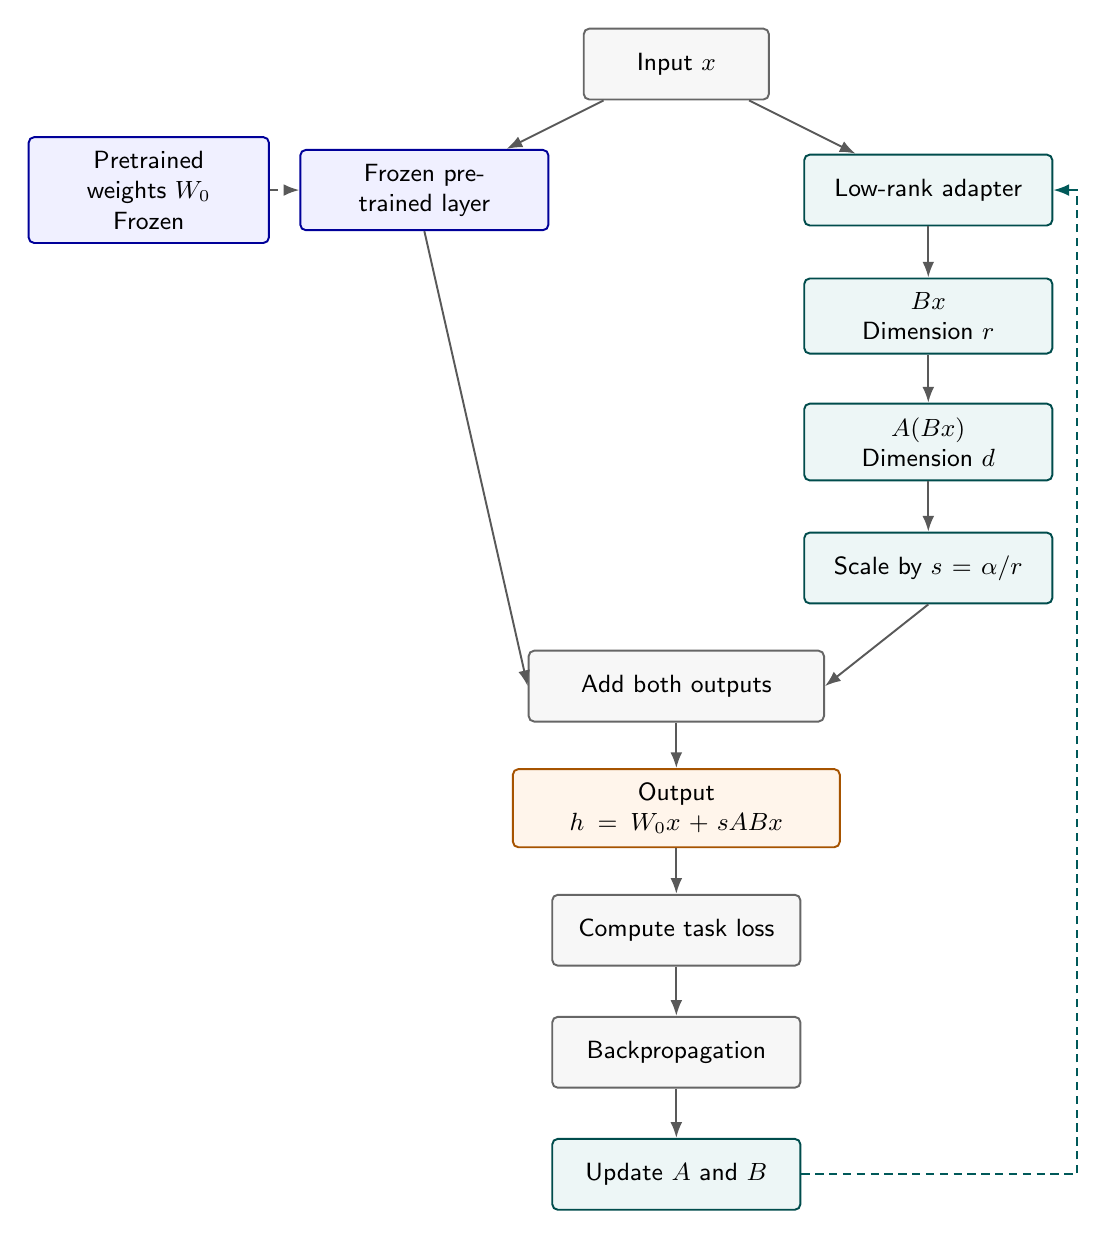
\begin{tikzpicture}[
  font=\sffamily\small,
  block/.style={
    draw=black!60,
    fill=black!3,
    rounded corners=2pt,
    line width=0.7pt,
    minimum height=9mm,
    text width=2.8cm,
    align=center,
    inner sep=5pt,
  },
  frozen/.style={block, draw=blue!60!black, fill=blue!6},
  adapter/.style={block, draw=teal!60!black, fill=teal!7},
  result/.style={block, draw=orange!65!black, fill=orange!8},
  arrow/.style={draw=black!65, line width=0.7pt, -{Latex[length=2mm]}},
  frozen-link/.style={arrow, densely dashed},
  feedback/.style={arrow, densely dashed, draw=teal!70!black},
]

% Input branches into the frozen base layer and trainable low-rank adapter.
\node[block, text width=2.0cm] (input) at (0,0) {Input \(x\)};
\node[frozen] (base) at (-3.2,-1.6) {Frozen pretrained layer};
\node[adapter] (lowrank) at (3.2,-1.6) {Low-rank adapter};
\node[frozen, text width=2.7cm] (weights) at (-6.7,-1.6)
  {Pretrained weights \(W_0\)\\Frozen};

\draw[arrow] (input) -- (base);
\draw[arrow] (input) -- (lowrank);
\draw[frozen-link] (weights.east) -- (base.west);

% Low-rank path and sum with the frozen layer output.
\node[adapter] (bproj) at (3.2,-3.2) {\(Bx\)\\Dimension \(r\)};
\node[adapter] (aproj) at (3.2,-4.8) {\(A(Bx)\)\\Dimension \(d\)};
\node[adapter] (scale) at (3.2,-6.4) {Scale by \(s = \alpha/r\)};
\node[block, text width=3.4cm] (sum) at (0,-7.9) {Add both outputs};

\draw[arrow] (lowrank) -- (bproj);
\draw[arrow] (bproj) -- (aproj);
\draw[arrow] (aproj) -- (scale);
\draw[arrow] (base.south) -- (sum.west);
\draw[arrow] (scale.south) -- (sum.east);

% Loss and optimization update only the low-rank matrices.
\node[result, text width=3.8cm] (output) at (0,-9.45)
  {Output\\\(h=W_0x+sABx\)};
\node[block] (loss) at (0,-11.0) {Compute task loss};
\node[block] (backprop) at (0,-12.55) {Backpropagation};
\node[adapter] (update) at (0,-14.1) {Update \(A\) and \(B\)};

\draw[arrow] (sum) -- (output);
\draw[arrow] (output) -- (loss);
\draw[arrow] (loss) -- (backprop);
\draw[arrow] (backprop) -- (update);
\draw[feedback] (update.east) -- ++(3.5,0) |- (lowrank.east);
\end{tikzpicture}
\end{document}
